
\documentclass[journal]{IEEEtran}

\usepackage{array}
\usepackage{graphicx}
\ifCLASSINFOpdf
 
\else
 
\fi



\hyphenation{op-tical net-works semi-conduc-tor}


\begin{document}

\title{ Congestion Notifier\\ Do not wandering around anymore}


\author{ Kim Jihun(2014005432),~\IEEEmembership{Information System,Hanyang Univ,}\\
        Park Junhyeong(2015005487),~\IEEEmembership{Information System,Hanyang Univ,}
        \\and~Jeong Seunghwan(2013021823),~\IEEEmembership{Information System,Hanyang Univ,}% <-this % stops a space
\thanks{M. Shell was with the Department
of Electrical and Computer Engineering, Georgia Institute of Technology, Atlanta,
GA, 30332 USA e-mail: (see http://www.michaelshell.org/contact.html).}% <-this % stops a space
\thanks{J. Doe and J. Doe are with Anonymous University.}% <-this % stops a space
\thanks{Manuscript received April 19, 2005; revised August 26, 2015.}}









% make the title area
\maketitle

% As a general rule, do not put math, special symbols or citations
% in the abstract or keywords.
\begin{abstract}
In many cases, some places like café, library or restaurant is not available because there are too many people so no space inside. This forces people additional effort to find somewhere else. To avoid this annoying situation, we make a congestion notifier which informs whether the places are available or not before people actually visit there. We will use censors and Arduino for the process of counting the number of people who get in or out the place. Based on this number, we calculate congestion level and then notify the results who needs this information. we will also provide related information which users can look as references. Expected time congestion level drops, average congestion level on specific place during recent one week and recent congestion level on specific place during specific time(lunch, dinner time). To calculate these information we will process counting censor value via several internal algorithms. Then recommendation on place that which place is most suitable for visit among several candidates will be provided for users. The menu of the restaurant or café will be included. There will be request board in which users can leave opinion about the app after using it such as error of the applications or some other functions they wish this app provides.
\end{abstract}

% Note that keywords are not normally used for peerreview papers.
\begin{IEEEkeywords}
IEEE, IEEEtran, journal, \LaTeX, paper, template.
\end{IEEEkeywords}





\IEEEpeerreviewmaketitle









\section*{Role Assignments}\\

%\begin{center}

%\begin{tabular}{ | m{5em} | m{1cm}| m{1cm} | } 
%\bfseries Roles & \bfseries Name & \bfseries Task description and etc\\
%\hline
%cell1 dummy text dummy text dummy text& cell2 & cell3 \\ 
%\hline
%cell1 dummy text dummy text dummy text & cell5 & cell6 \\ 
%\hline
%cell7 & cell8 & cell9 \\ 
%\hline
%\end{tabular}
%\end{center}



\begin{table}[h]

\renewcommand{\arraystretch}{2.3}
%\caption{A Simple Example Table}
%\label{table_example}
\centering
\begin{tabular}{ | m{2cm} | m{1.5cm}| m{4cm} | } 
\hline
\bfseries Roles & \bfseries Name & \bfseries Task description and etc\\
\hline

User\&Customer & Kim Jihun &Identify user requirements, Software feedback\\
\hline
Software Developer & Jeong Seunghwan&Implementation, source coding, testing\\
\hline
Development manager & Park Junhyeong & Project planning, Manage each development processes.\\
\hline
\end{tabular}
\end{table}



\section{Introduction}

\IEEEPARstart{W}{e} visit places like café, restaurant in daily life and sometimes we have no choice but to move out as there is simply no space or sets available inside. Wandering around to find somewhere else available nearby was really dissapponting especially when the weather was not good.
Our team wanted this kind of problems never happen again. So, we thought to put some counting censors near the entrance door and keep track of the number of people inside. If the place becomes crowded and no room for people, we change the congestion level from “available” to “not available”. Users can easily find out which place is least crowded among candidates by checking out recommendation of the app or related information such as Expected time congestion level drops. One they choose the place to visit users can also find the menu of that place from application. If there were some uncomfortableness while they use the app, they can leave some request messages on request board.   
	There are plenty of similar software tells users that the place you are heading is already crowded. For example, one of them notifies how many people is queueing for each departure gates of Incheon airport.(Naver- inchoen airport departure gate information) Another one informs how many students inside the student’s restaurant.(Yonsei University representative mobile app) 

% You must have at least 2 lines in the paragraph with the drop letter
% (should never be an issue)

%여기에 뭐엏어야댐?????
%\hfill mds
%작자같은거 쓰는 코드인가? 
%\hfill August 26, 2015

% 이코드쓰면 에이비씨디 나옴.
%  \subsection{Subsection Heading Here}
%Subsection text here.

% needed in second column of first page if using \IEEEpubid
%\IEEEpubidadjcol
%이 코드쓰면 숫자나옴.
%\subsubsection{Subsubsection Heading Here}
%Subsubsection text here.







\section{REQUIREMENTS}

\subsection{Censors technique}
Need some sensors to count people in and out of specific place where we have chosen before.
\subsection{Arduino technique}
We will use Arduino to receive the measured censor value and send it to the server.
\subsection{Database}
We need some database to store censor data continue in short intervals. This database will be connected to server to support user interface web application.
\subsection{Server}
We need a web server to support a user web application. When the a button on user web page clicked server will send proper answer to client. Server will be connected to database which contains censor measurement data on each places.
\subsection{Web design}
We will build a website that users can access freely. 
 In the main page, the map of Hanyang University will be displayed as output of requirement J. On the map each student restaurant will be highlighted. On the lower part of the main page outputs of requirement L and simple button to support requirement N will be displayed. When user click one restaurant on the map, detail page of the restaurant will come out. The detail page should contain information of requirement F, G, H, I and simple button to support requirement L. 

\subsection{Current congestion level }
We will provide current congestion level with percentage or some linear order(high, normal, low).
\subsection{Expect time to congestion level drops}
If the congestion level or percentage is high on certain space, how much time you need to wait for congestion level drop will be displayed.
\subsection{Average congestion level on specific place}
The average congestion level for week will be provided on each place detail web pages. 
\subsection{Congestion level in specific time}
Average congestion level of the place in specific time will be displayed. For example, congestion level of restaurant A in lunch time and dinner time.
\subsection{Show location on GPS}
Show physical location of each place such as student’s restaurant on the GPS map. Each place on the map should support hypertext link which delivers users detail page which include information of which is output of requirement F, G, H and I.
\subsection{Restaurant Information}
On detail page described in requirements J, a section that provides information about menus and prices of restaurants will be included.
\subsection{Request board- opinion for application itself}
In the lower part of the main page, some text hyperlink will be provided. On detail page of this hyperlink, users can post their opinion such as inconvenience they felt during usage or request of new functions that they wish our service support.
\subsection{Request board- opinion for each restaurant}
In the detail page of each restaurant, users can leave some comments regarding that specific restaurant. Those can be assessment of that restaurant menu or any trivial points which writer want to inform other users.  
\subsection{Recommendation}
Recommendation among restaurants where congestion level is lowest among candidates. This information will be shown at the main page so that users quickly decide which place they should go. 

%Subsection text here.

\section{DEVELOPMENT ENVIRONMENT}

\subsection{Choice of software development platform}
Operating system
- windows 10 Home 64bit, ubuntu-16.04.2-desktop-amd64

Computer resources
- Intel(R) Core(TM) i5-5200u CPU @ 2.20GHz, 8.00GB RAM\\
- Intel(R) Core(TM) i5-4210U CPU @ 1.70GHz 2.40GHz,  RAM: 8.00GB\\
- Intel(R) Core(TM)i5-6200U CPU @ 2.30GHz 2.40 GHz, RAM: 8.00GB\\

Commercial cloud platform\\
- Firebase is a Backend-as-a-Service—BaaS—app-development platform on Google Cloud Platform.
Choice reason: It provides easy way of backend development process and real time database.\\


Programing language\\
- node.js 
Choice reason: to develop server via Firebase, node.js installation is prerequisite of Firebase.
-Angular.js
Choice reason: to apply Javascript function. Angular.js is  a Javascript Framework. It can be added to an HTML page with a <script> tag.
-AngularFire 
Choice reason: AngularFire connects angular.js to Firebase service.
-html5, css3
Choice reason: to develop web front end.
-Arduino sketch
Choice reason: to process censor values which counts the number of people in or out. To send http request to Firebase realtime database.\\

Cost estimation\\
- Operating system

Windows 10 Home: free validation key is available from Hanyang University student information center.

ubuntu-16.04.2-desktop-amd64:: Open source free ware.

-Firebase
Free charge service(Spark charge plan) would be enough to do this project. We can use 1G cloud and database storage.

-Arduino board
1 copy of Yun board which is approximately 96\$. 
Choice reason: Yun internally contains linux server and wifi shield so that it can be connected to internet and send HTTP request directly to Firebase.

-Circuit elements
 registers with various range of resistance value, radio censors, connecting wires, small breadboard. All of these costs less than 10\$.

\subsection{Software in use}
There are plenty of similar software tells users that the place you are heading is already crowded. For example, one of them notifies how many people is queueing in front of each departure gates of Incheon airport.(Naver- inchoen airport departure gate information) Another one informs how many students inside the student’s restaurant.(Yonsei University representative mobile app) 




\section{SPECIFICATOIN}


\subsection{Requirement A- Censors technique.}
We will attach two pair of radio censors near the entrance door to support bidirectional people counting. If the first pair of radio censor detect a person and then the second pair detect a person, this means that that person came in the room. If the pair of censors detected a person in reverse order, this means that a person is going out. Whenever people get in the counting number increases, and gets out the number decreases. That number will be passed to data base continuously soon after the number changes.
\subsection{Requirement B-  Arduino technique}
Small breadboard will be connected to Arduino to build up electrical circuits. Electric components such as register, censer, wires, battery will be included. Arduino Yun which contains independent Wifi shield and linux server component will process radio censor values and subsequently send HTTP request to database in our case Firebase real time server.
\subsection{Requirement C- Database}
we need to reflect congestion level(censor value) of each restaurant to our web application real time. So we chose the Firebase real time database which is a cloud-hosted NoSQL database that lets you store and sync data between your users in real time. Data will be stored in JSON format.
\subsection{Requirement D- Server}
The sever updates the main page whenever the congestion level of each restaurant changes. When each restaurant on the map clicked, the server send the detail page of its own to web browser. When the request button on lower part of the main page is clicked the server returns request board(for application itself) page to Web browser.
\subsection{Requirement E- Web design}
On the main page there will be Hanyang University’ map on the middle of the screen. Students restaurants on the map will be pointed out with some pictures and those are options for users. Under the map the link button to request board(for applicaton itself) will be placed. Detail page of request board(for application itself) consist of only lists of user comment about the app.  Upper part of the map in the main page, recommendation of current least crowded restaurant will be shown. Users can click one restaurant on the map that they want to know its congestion level. When certain restaurant is click on the main page, the corresponding detail page will come out. The detail page displays information produced from requirement F, G, H, I and K in either plain text or tabular form. Above the arrow indicating each restaurant on the map, current congestion level will be provided so users can easily compare the candidate based on their location. 
%그림넣는코드 

\begin{figure}[h]
\centering
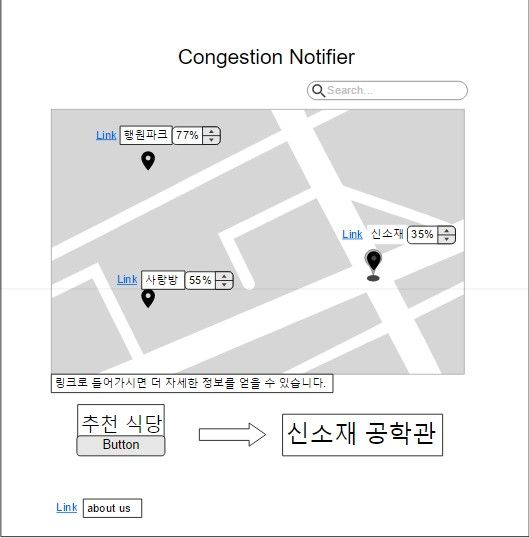
\includegraphics[scale=0.5]{mainpage.jpg}
\caption{Main page}
\label{fig:Main page}
\end{figure}

\begin{figure}[h]
\centering
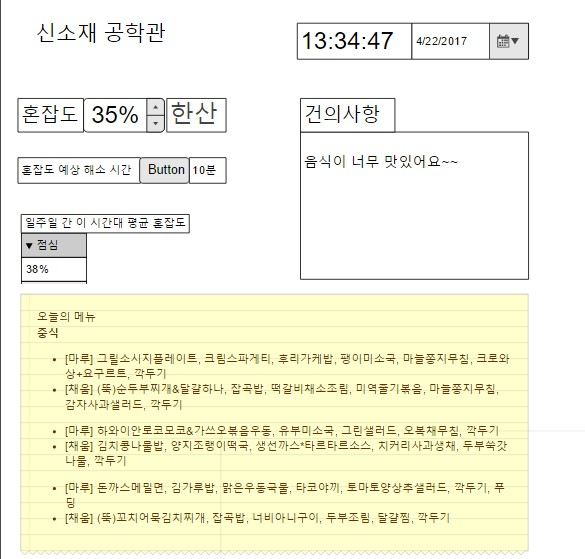
\includegraphics[scale=0.5]{detailpage.jpg}
\caption{Detail page}
\label{fig:Detail page}
\end{figure}

\subsection{Requirement F- Current congestion level }
Current congestion level will be calculated in ratio. Each restaurant certainly have the maximum number of people which they can accommodate. The number of people who actually in the restaurant will be divided by the maximum number of people of certain restaurant and this value will be multiplied by 100 to convert it percentage value.
\subsection{Requirement G- Expect time to congestion level drops}
Using each restaurant’s 1 week congestion level record, we will keep track of how much time it will take high congestion level turn in to lower level. If the congestion level or percentage is low or medium on certain space, nothing will be displayed.
\subsection{Requirement H- Average congestion level on specific place}
We will save congestion level of specific restaurant every 1 hour. Based on that data we will compute 1 day’s overall congestion level. If “high” was most frequently among 24 data(1 congestion level per l hour), that day’s congestion level is “high”. On the same manner based on 1 day’s congestion level in recent 1 week, we can compute 1 week’s congestion level of specific place.
\subsection{Requirement I- Congestion level in specific time}
First total number of visitors who visited during specific time such as lunch or dinner in recent 1 week will be calculated by adding the number of each day’s visitors of specific restaurant in specific time. Then divided that number by 7 to calculate average visitors during that  period of time. Finally divide average visitors during specific time by maximum number of people that the specific restaurant can accommodate to calculate congestion level in specific time of specific restaurant.
\subsection{Requirement J- Show location on GPS.}
On the map the location of the restaurant will be pointed by downward arrow. Current congestion level will be displayed right on the arrow in tiny simple box. Then when user clicks the arrow or the box, detail page of that location will be served. That detail page should contain output of requirement F, G, H and I.
\subsection{Requirement K- Restaurant Information}
On detail page described in requirements J, a section that provides menu and price information of restaurants will be included. These information will be presented as text and picture of the menu will not be included.

 And whoever use the restaurant can write whatever they want to do in restaurant’s board. the limitation of restaurant’s textbox is under 500 words. The word’s font is fixed in gothic style. 

\subsection{Requirement L- Request board- opinion for application itself}
In the lower part of the main page, some text hyperlink will be provided. On detail page of this hyperlink, users can post their opinion such as uncomfortableness they felt during usage or request of new functions that they wish our service to support. 
User comments should be saved in database so the administer can use this comment to further develop our application. The length of comment will be restricted up to 1000 characters. Newest comment will be shown at the top position of the board just like stacks.

\subsection{Requirement M- Request board- opinion for each restaurant}
In the detail page of each restaurant, users can leave some comments regarding that specific restaurant. Those can be assessment of that restaurant menu or any trivial points which writer want to inform other users.  


In the detail page of each restaurant, users can leave some comments regarding that specific restaurant. Comments can be of any subjects such as assessment of that restaurant menu or any trivial points which the writer want to inform other users. User comments should be saved in database so later the administer can hand over this comments to managers of the restaurants. The length of comment will be restricted up to 1000 characters. Newest comment will be shown at the top position of the board just like stacks.

\subsection{Requirement N- Recommendation}
Recommend on restaurants where congestion level is lowest among candidates. This information will be shown at the upper part of main page so that users quickly decide which place they should go. This task will be performed by comparing congestion levels of each restaurant or sort the congestion rate value in decreasing order. 




\section{ARCHITECTURE DESIGN \& IMPLEMENTATION}\\


\subsection{Overall architecture}


\begin{figure}[h]
\centering
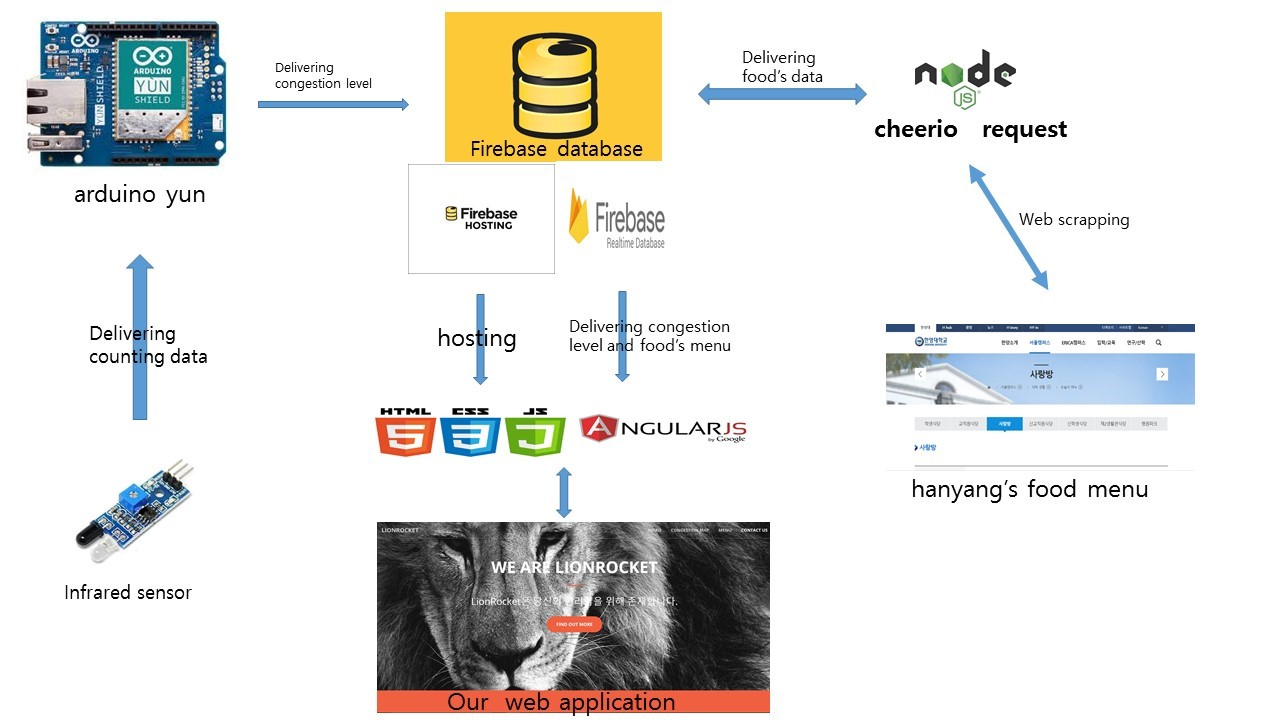
\includegraphics[scale=0.25]{map.jpg}
\caption{Main page}
\label{fig:Main page}
\end{figure}
\subsection{Directory organization}

%표녛기

\begin{table}[h]

\renewcommand{\arraystretch}{2.3}
%\caption{A Simple Example Table}
%\label{table_example}
\centering
\begin{tabular}{ | m{2cm} | m{1.5cm}| m{2.7cm} | m{0.5cm} |} 
\hline
\bfseries Directory & \bfseries File Names & \bfseries Module names in use & \bfseries Etc \\
\hline

Project/Arduino/ & Count.ino &Arduino Yun(ir sensor)&\\
\hline

Project/Firebase /functions  & node\_modules & Node.js,Firebase&\\
\hline

Project/Firebase /public  & Index.html &Html,Google mapapi, Angular Js&\\
\hline

Project/Firebase /public  & scraping.js &NPM\_request, cheerio(package)&\\
\hline

Project/Firebase /public  &Browserfied\_ scraping.js 

&NPM\_Browserify
(package)&\\
\hline

Project /Firebase/public
/css
 & Creative.css &Bootstrap
CSS
File
&\\
\hline

Project /Firebase/public
/img
 & Header.jpg, sum.jpg &Bootstrap
Image
(main page,
Thumb mail
Image)
&\\
\hline

Project /Firebase/public
/js
 &creative.js, creative.min.js&Bootstrap\_theme
Javascript file
&\\


\hline
\end{tabular}
\end{table}


\subsection{Module-Arduino Yun(ir sensor}
- Arduino yun:  \\
1. Receive ir sensor measurement value.
 If the first pair of ir sensors detect a person passing first increase count value by1. Likewise, if the other pair of ir sensors detect a person passing first then decrease count value by 1.

2. Send count value(current number of people inside) to firebase real- time data base server.
 As Arduino yun internally contains linux server and can be connect to internet network via wifi, it can get accurate time of Seoul via date() function. Arduino passes current count value and measurement time as one json node to firebase server via Curl command.
- ir sensor: consists of two pair of ir light transmitter and ir receiver. Each pair detects a person passing between them.

Source codes are in  Project/Arduino.

\subsection{Module 2(Node.js, firebase}
1. Node.js – sever side language based on javascript.
 
2.Firebase -google’s overall development service which provide real-time database and web hosting service.
 
We chose firebase as it enables easy deployment of web application. Node. js is prerequisite of firebase hosting service. Source files are in Project/Firebase/functions. 

\subsection{Module3(NPM package-request,cheerio,curl}
These modules are used to show hanyang university restaurant menu on web page.

NPM package -request, cheerio: Access hanynag university restaurant’s website and scrape the menu in string. Installed by cmd command “npm install request cheerio curl”

NPM package -curl: used to post restaurant menu as a string to firebase database in json format {“Menu”  : “Soup….” }
Source code location is Project/Firebase/public/scraping.js

\subsection{Module4(Bootstrap CSS templete}
Bootstrap CSS template is implemented to construct web-front end. Instead of building web front end on our own, we chose to adopt Bootstrap template because all members are not good at web front end design and it is time saving. 
Source code location is Project /Firebase/public/Creative.css

\subsectio{Module 5(Header.jpg, sum.jpg}
Header.jpg is a picture which decorates web application’s main page. Sum.jpg is a thumbnail image that shows up when someone sends our website’s URL as kakaotalk message.
\subsection{Bootstrap theme javascript file}
Bootstrap theme javascript file: javascript file that support bootstrap theme.
Source code location is Project /Firebase/public/js .

\section{USE CASE}


%1번
\subsection{Check congestion level}
1.Access “our url-(not specified yet)” \\
2.Click the Congestion-Map button on the right top\\
\begin{figure}[h]
\centering
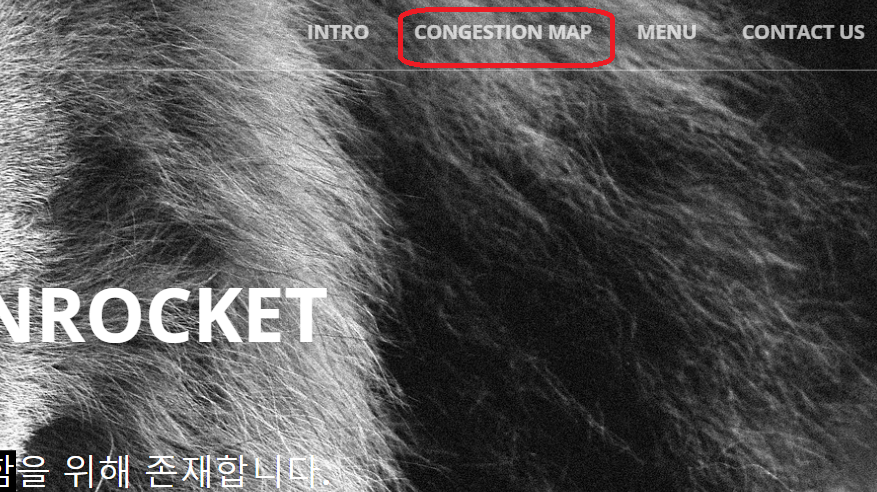
\includegraphics[scale=0.5]{congestion.png}
\caption{congestion button}
\label{fig:congestion button}
\end{figure}

\\3.Verify the congestion level

\begin{figure}[h]
\centering

\includegraphics[scale=0.5]{1.jpg}
\caption{congestion level}
\label{fig:congestion level}
\end{figure}


\\


%2번
\subsection{Check location of restaurant}
1. Access “our url-(not specified yet)” \\
2. Click the Congestion-\_Map button on the right top. 
\begin{figure}[h]
\centering
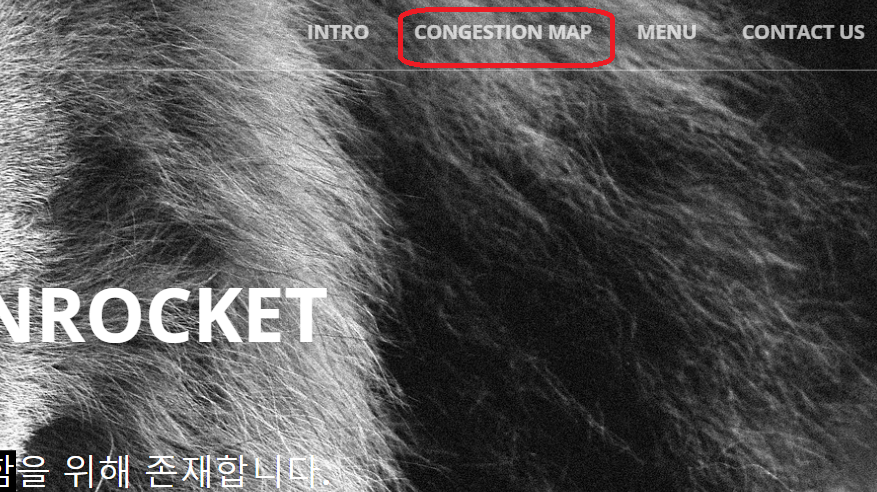
\includegraphics[scale=0.5]{congestion.png}
\caption{congestion button}
\label{fig:congestion button}
\end{figure}
\newline
\newline
\newline
\newline
\newline
\\3. Check the location of the restaurant on the map.

\begin{figure}[h]
\centering
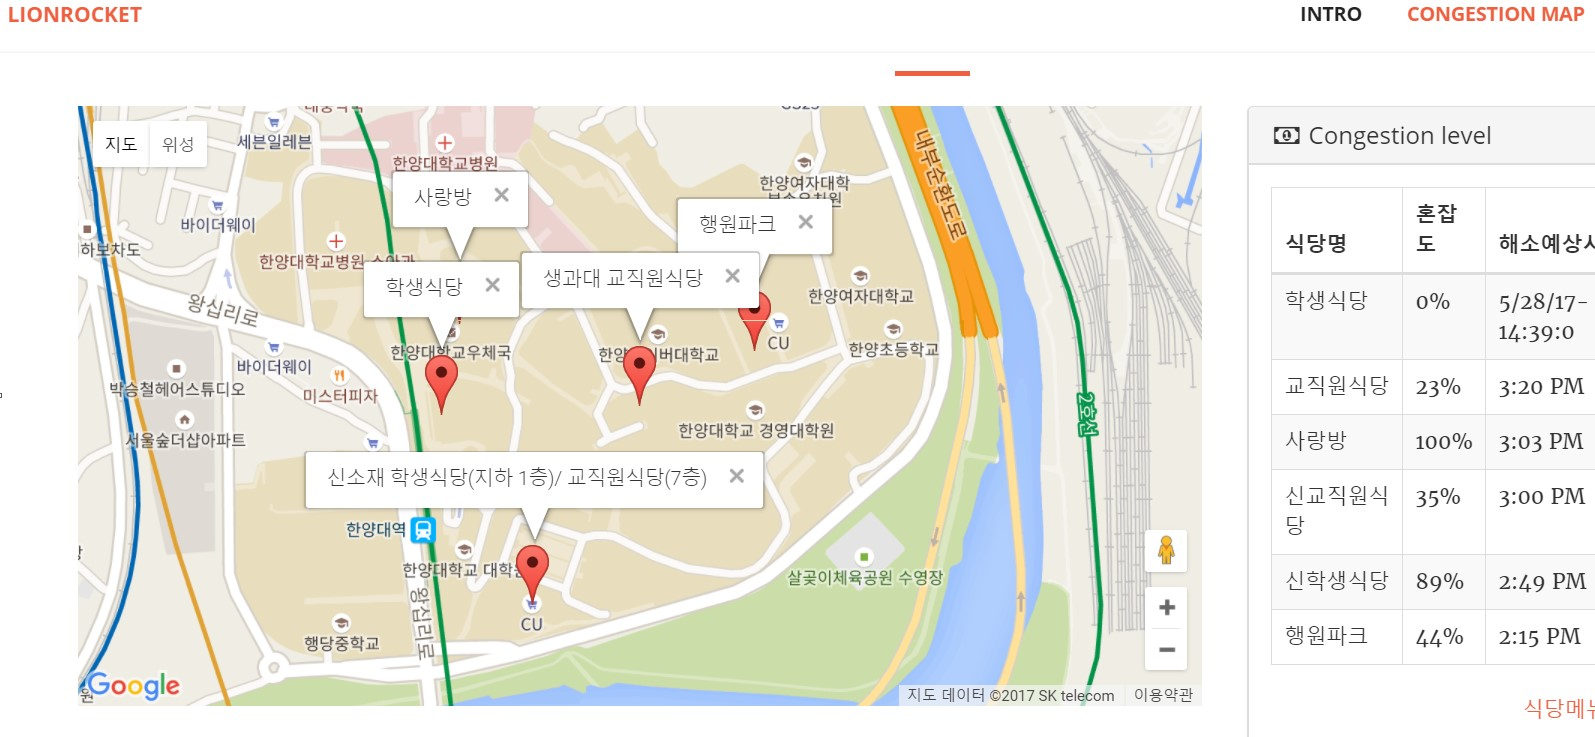
\includegraphics[scale=0.17]{B.jpg}
\caption{congestion map}
\label{fig:congestion button}
\end{figure}



% C 번
\subsection{Check estimated amount time which takes congestion
level drops to normal or below}
\newline1. Access “our url-(not specified yet)”\\   2. Click the Congestion Map button on the right top.
\newline
\begin{figure}[h]
\centering
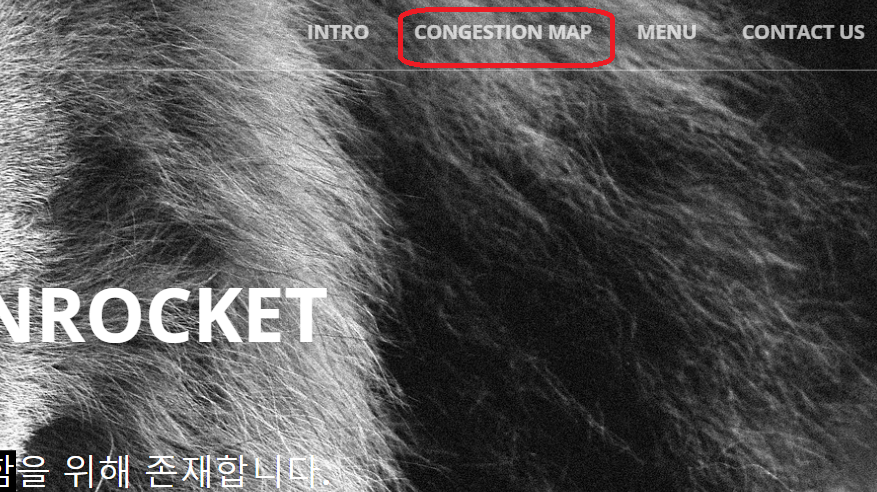
\includegraphics[scale=0.5]{congestion.png}
\caption{congestion button}
\label{fig:Main page}
\end{figure}

\newline


3. Check estimated time to congestion level drop\\
\newline\newline\newline\newline\newline\newline\newline
\newline
\newline
\newline
\begin{figure}[h]
\centering
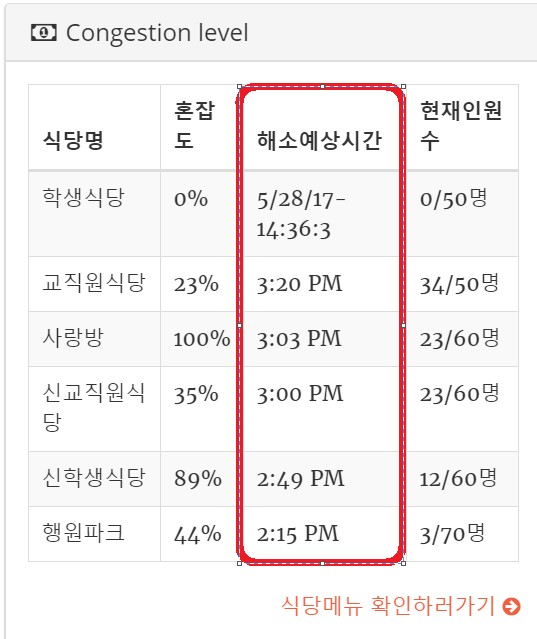
\includegraphics[scale=0.4]{C.jpg}
\caption{congestion button}
\label{fig:Main page}
\end{figure}

%D번
\newline
\subsection{Check restaurant's menu}
1. Access “our url-(not specified yet)” \\
2. Click the Congestion\_Map button on top right.\\

\begin{figure}[h]
\centering

\includegraphics[scale=0.3]{E1.jpg}
\caption{Main page}
\label{fig:congestion button}
\end{figure}

\newline
3.Check restaurant’s menu
\newline\newline\newline\newline\newline\newline\newline
\newline\newline\newline\newline\newline\newline\newline\newline
\newline\newline\newline\newline\newline\newline\newline

\begin{figure}[h]
\centering
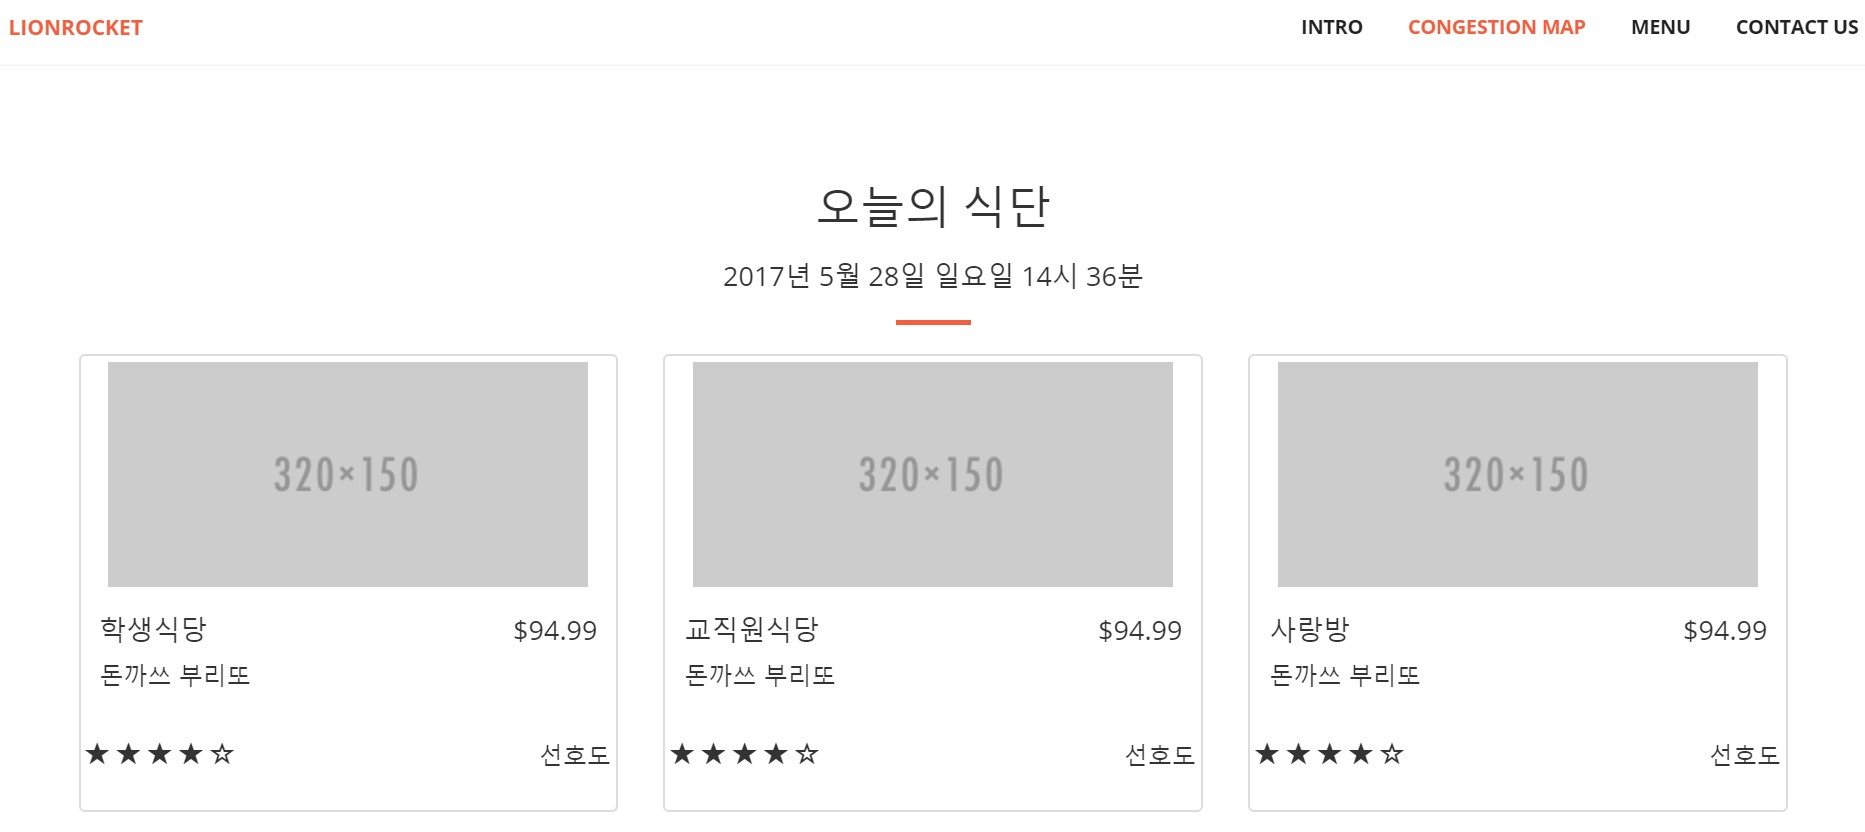
\includegraphics[width=3in,height=2in]{E2.jpg}
\caption{Main page}
\label{fig:congestion button}
\end{figure}


%E번

\subsection{Contact to developers}
1. Access “our url-(not specified yet)”
2. Click the Contact Us button on the right top.
\begin{figure}[h]
\centering

\includegraphics[scale=0.3]{F1.jpg}
\caption{Main page}
\label{fig:congestion button}
\end{figure}




3. Confirm phone number and email address of developers.    
\begin{figure}[h]
\centering
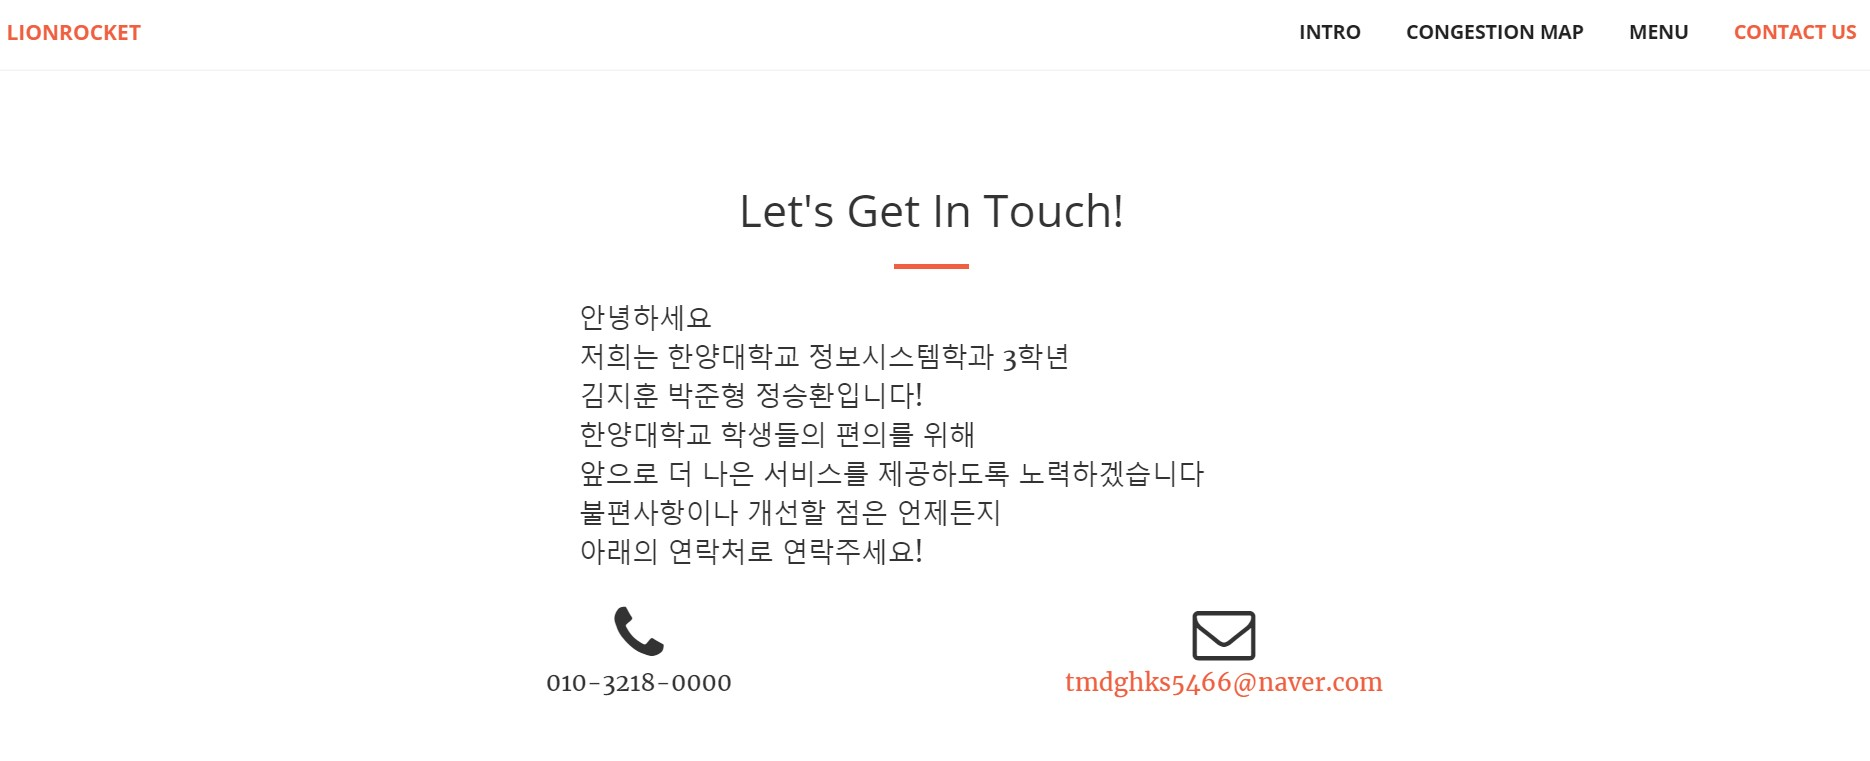
\includegraphics[scale=0.2]{F2.jpg}
\caption{Main page}
\label{fig:congestion button}
\end{figure}

4. Contact to developers.







\end{document}


